\smalltitle{سوال 1}\\
\begin{enumerate}[wide, labelwidth=!, labelindent=0pt]
    \item کافی است که به راحتی چهار نقطه‌ی بر روی صفحه انتخاب کنیم. در این صورت هر دو نقطه‌ی را که در نظر
بگیریم، خط گذرنده از آن‌ها بر صفحه‌ی
$P$ است. یک سری از این نقاط به صورت زیر هستند:
\begin{equation*}
    (9, 0, 0), (7, 1, 0), (5, 2, 0), (3, 3, 0)
\end{equation*}
    \item مشخص است که شکل حاصل یک سهمی ناقص است بعلاوه‌ی یک نقطه. شکل رسم شده‌ی آن‌ها را می‌توانید در زیر مشاهده‌کنید:
\begin{figure}[H]
    \centerline{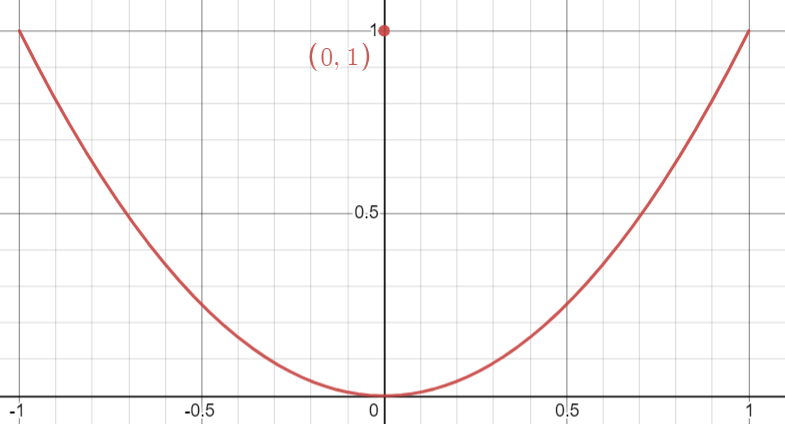
\includegraphics[scale=.3]{source/1-2-1.png}}
\end{figure}
\noindent
حال برای کشیدن
\lr{convex-hull}
باید شکلی محدب بکشیم که کل نمودار ما را شامل باشد. پس کافی است که علاوه بر سهمی، پاره خطی از
دو سر انتهایی سهمی رسم کنیم که نقطعه‌ی
$(0,1)$
را نیز شامل بشود مانند شکل زیر:
\begin{figure}[H]
    \centerline{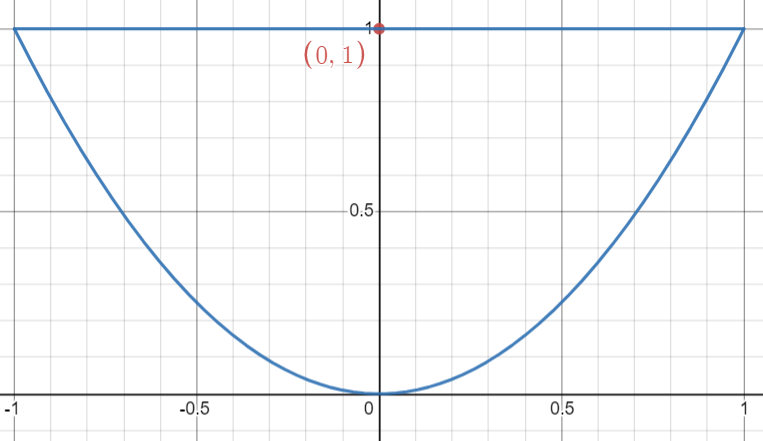
\includegraphics[scale=.3]{source/1-2-2.png}}
\end{figure}
    \item در ابتدا بررسی می‌کنیم که آیا
$v_i$ها
ترکیب خطی یکدیگر هستند یا خیر. برای این کار معادله‌ی زیر را حل می‌کنیم:
\begin{align*}
    \begin{array}{r@{\mskip\thickmuskip}l}
		100 &= 2\alpha_1 + 2\alpha_2 + 0\alpha_3\\
		-100 &= 6\alpha_1 + 2\alpha_2 -99\alpha_3\\
		400 &= -8\alpha_1 -4\alpha_2 + 33\alpha_3
    \end{array}
    \implies
    \begin{array}{r@{\mskip\thickmuskip}l}
        100 &= 2\alpha_1 + 2\alpha_2\\
        1100 &= -18\alpha_1 - 10\alpha_2
    \end{array}
    \implies
    \begin{array}{r@{\mskip\thickmuskip}l}
        \alpha_1 = -200\\
        \alpha_2 = 250\\
        \alpha_2 = -\frac{200}{33}\\
    \end{array}
\end{align*}
پس این بردار‌ها ترکیب خطی یکدیگر هستند. پس می‌توان نوشت:
$v_4 = -200v_1 + 250v_2 -\frac{200}{33}v_3$
حال
$y$
را بر حسب
$v_1, v_2, v_3, v_4$
می‌نویسیم:
\begin{align*}
y &= \alpha_1 v_1 + \alpha_2 v_2 + \alpha_3 v_3 + \alpha_4 v_4\\
&= \alpha_1 v_1 + \alpha_2 v_2 + \alpha_3 v_3 + \alpha_4 ( -200v_1 + 250v_2 -\frac{200}{33}v_3 )\\
&= (\alpha_1 - 200\alpha_4) v_1 + (\alpha_2 + 250\alpha_4) + (\alpha_3 - \frac{200}{33}\alpha_4) v_3
\end{align*}
\begin{align*}
    \begin{array}{r@{\mskip\thickmuskip}l}
		1 &= 2(\alpha_1 - 200\alpha_4) + 2(\alpha_2 + 250\alpha_4) + 0(\alpha_3 - \frac{200}{33}\alpha_4)\\
		-1 &= 6(\alpha_1 - 200\alpha_4) + 2(\alpha_2 + 250\alpha_4) -99(\alpha_3 - \frac{200}{33}\alpha_4)\\
		2 &= -8(\alpha_1 - 200\alpha_4) -4(\alpha_2 + 250\alpha_4) + 33(\alpha_3 - \frac{200}{33}\alpha_4)\\
        1 &= \alpha_1 + \alpha_2 + \alpha_3 + \alpha_4
    \end{array}
\end{align*}
به کمک ماشین حساب این معادله را حل می‌کنیم و به جواب زیر می‌رسیم.
\begin{gather*}
    a_1 = -2.25\\
    a_2 = 3.31\\
    a_3 = -0.05\\
    a_4 = -0.01
\end{gather*}
% 1=2*(a_1-200*a_4)+2*(a_2+250*a_4),
% -1=6*(a_1-200*a_4)+2*(a_2+250*a_4)-99*a_3+600*a_4,
% 2=-8*(a_1-200*a_4)+33*a_4-200*a_4,
% a_1+a_2+a_3+a_4=1
پس یک ترکیب خطی
\lr{affine}
برای ساخت
$y$
وجود دارد.
    \item بله. به معادله‌ی زیر توجه کنید:
    \begin{align*}
        \begin{array}{r@{\mskip\thickmuskip}l}
            4 &= a + b\\
            1 &= ai_1 + bi_2
        \end{array}
        \implies
        1 = ai_1 + 4i_1 - ai_2
        \implies
        a = \frac{1 - 4i_1}{i_1 - i_2}
    \end{align*}
    تنها زمانی
    $a$
    جواب ندارد که
    $i_1 = i_2$
    باشد که یعنی یک بردار را انتخاب کنیم.
\end{enumerate}